\newpage
\chapter{Experimental Results}
\label{experiment_results}
\lhead{\emph{Experimental Results}}
We first present a full replication and extension of the work by
\citet{radDeliberationSinglePeakednessCoherent2021}. Then we present the simulations based on our model of
meta-deliberation, as well as the results of the sensitivity analysis on both
models. All code for the replication, main experiment and visualizations can be
found in \href{https://github.com/amirsahrani/master_thesis}{this Repository}.


\section{Replication} We are able to fully replicate the results found by
\citet{radDeliberationSinglePeakednessCoherent2021},  in \Cref{fig:rep_cyclic}
we see that while the bias is less than 0.73, all metric results in a-cyclic
preferences. We also replicate the behavior of the KS metric, where biases in
the range of 0.73-0.85, show even some initial a-cyclic profiles can become
cyclic. \Cref{fig:rep_count} Further explains this by showing that within this
range we always observe 3 unique profile for the KS metric, while DP and CS
have already settled on 6 profiles, thereby representing all possible
preferences. \Cref{fig:rep_condorcet} shows KS introduces ambiguity in the case
that there was a Condorcet winner, resulting in losing the original nice
profile. Finally, the proximity to single-peakedness shows a slightly more
positive note for the KS metric, showing that while the DP and CS bottom out to
the minimum proximity to single-peakedness, KS stays relatively close. Though
this should be taken with a grain of salt, as it is likely a consequence of the
unique preferences being smaller.

\begin{figure}[htbp]
	\centering
	\begin{minipage}{0.45\textwidth}
		\centering
		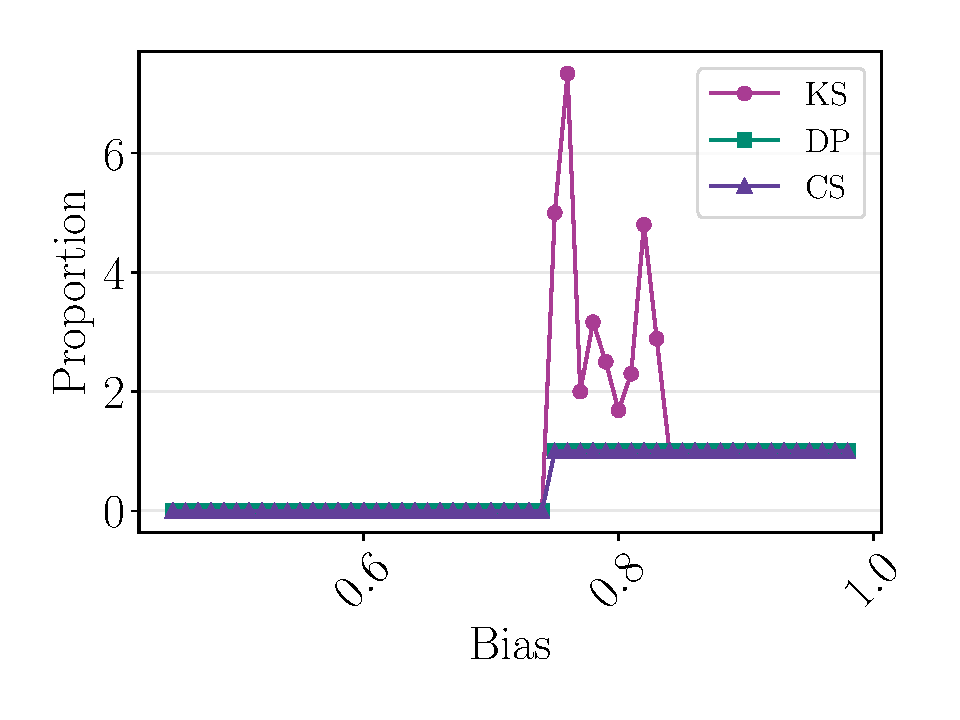
\includegraphics[width=\textwidth]{Figures/cyclic_proportion_Proportion.pdf}
		\caption{The proportion of cyclic profiles remaining, 0 indicating that no cyclic profiles were present after deliberation.}
		\label{fig:rep_cyclic}
	\end{minipage}\hfill
	\begin{minipage}{0.45\textwidth}
		\centering
		\vspace{-9pt}
		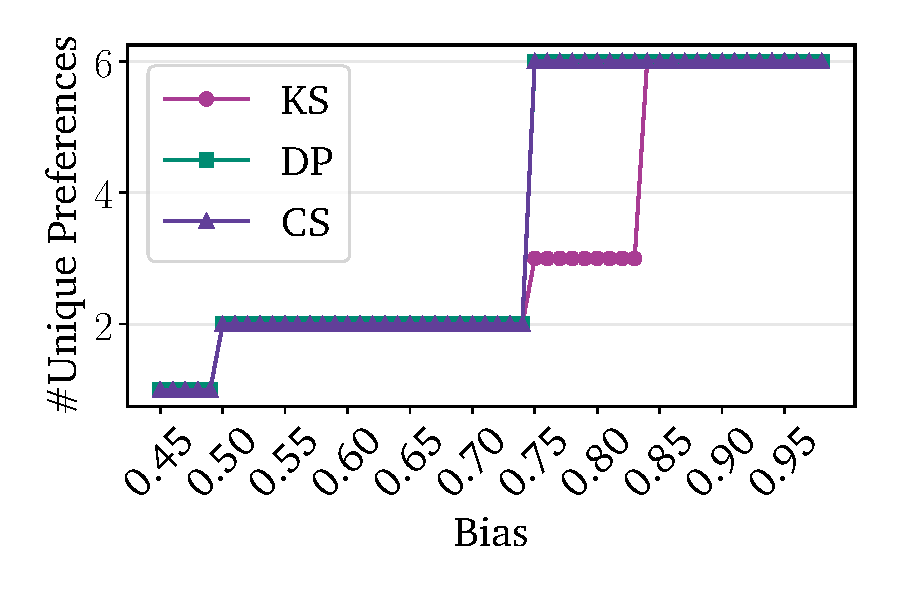
\includegraphics[width=\textwidth]{Figures/unique_Unique Preferences.pdf}
		\caption{Number of unique preferences at the final step of deliberation.}
		\label{fig:rep_count}
	\end{minipage}

	\vspace{1em}

	\begin{minipage}{0.45\textwidth}
		\centering
		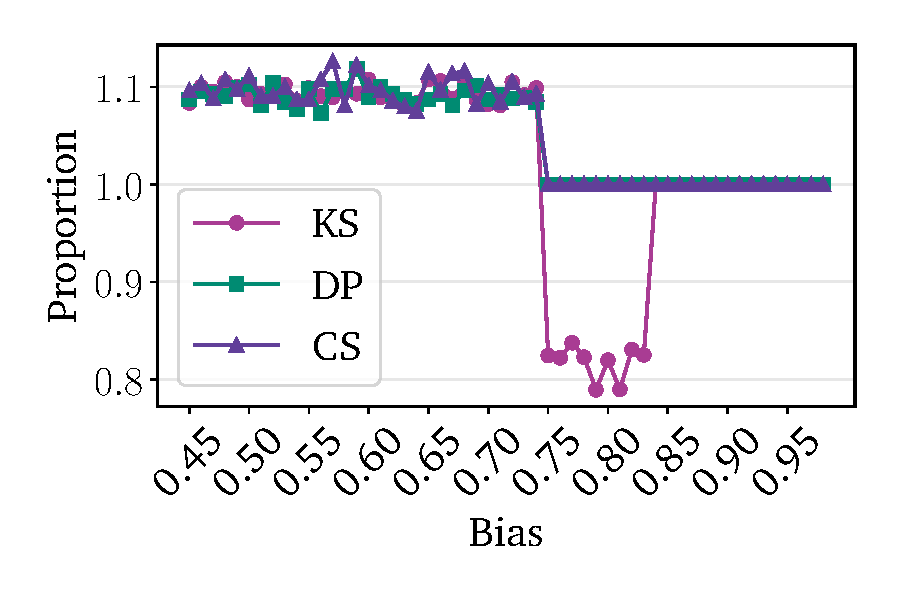
\includegraphics[width=\textwidth]{Figures/condorcet_proportion_Proportion.pdf}
		\caption{The proportion of Condorcet winners left after deliberation, value above one indicate Condorcet winners emerging during deliberation}
		\label{fig:rep_condorcet}
	\end{minipage}\hfill
	\begin{minipage}{0.45\textwidth}
		\centering
		\vspace{-9pt}
		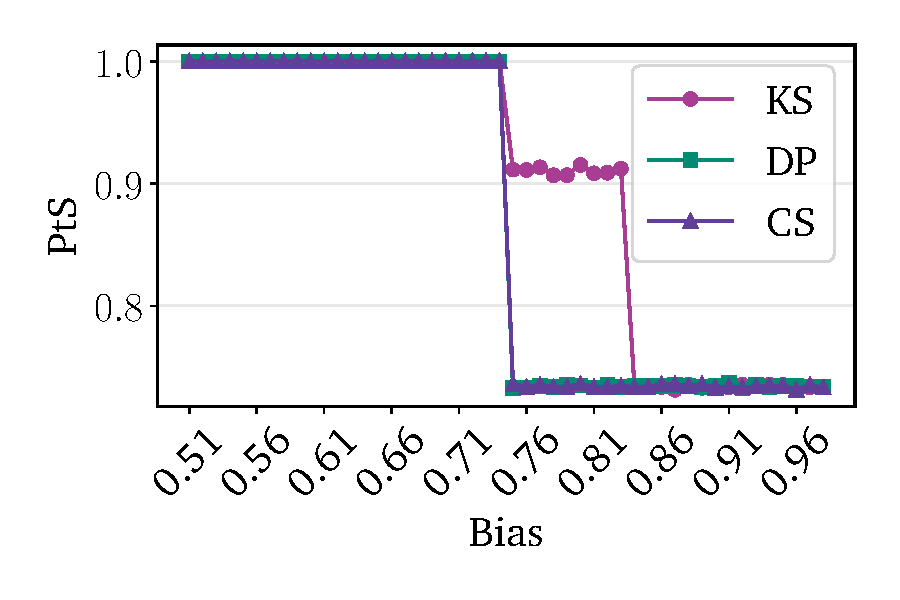
\includegraphics[width=\textwidth]{Figures/sp_proximity_PtS.pdf}
		\caption{Proximity to single-peakedness after deliberation. Proximity to single-peakedness as defined in \Cref{section:related_work}.}
		\label{fig:rep_single_peaked}
	\end{minipage}
\end{figure}
\newpage

\section{DeGroot Model} \label{degroot_results} \subsection{PBS Scores} We
first proceed with analyzing the performance of the DeGroot model on
substantive agreement. \Cref{fig:pbs} shows the PBS scores of both the
deliberation and control group, and the simulation results for both instances.
As expected the model performs poorly at predicting the control group, as
there was no significant change for control group members. Similar to the
control group, the starting PBS score of the participants is a strong
indicator for their PBS score. Therefore the model at t=0 is already
reasonably aligned with the final PBS scores. We see that after the first time
step the PBS scores get predicted more accurately, after which the model
starts making larger prediction errors. This is because the model keeps
averaging all opinions until a steady state is reaches in which most voters
hold non-extreme positions. Whether this is positive depends on
reality, as \citet{elsterMarketForumThree2002} remarked, if deliberation is
able to reach full consensus, the model might give a glimpse into how this
works. If this is not the case however, then the model is overly naive
suggesting that people come to hold a weighted average of all original
opinions. The latter seems more likely.


\begin{figure}
	\begin{center}
		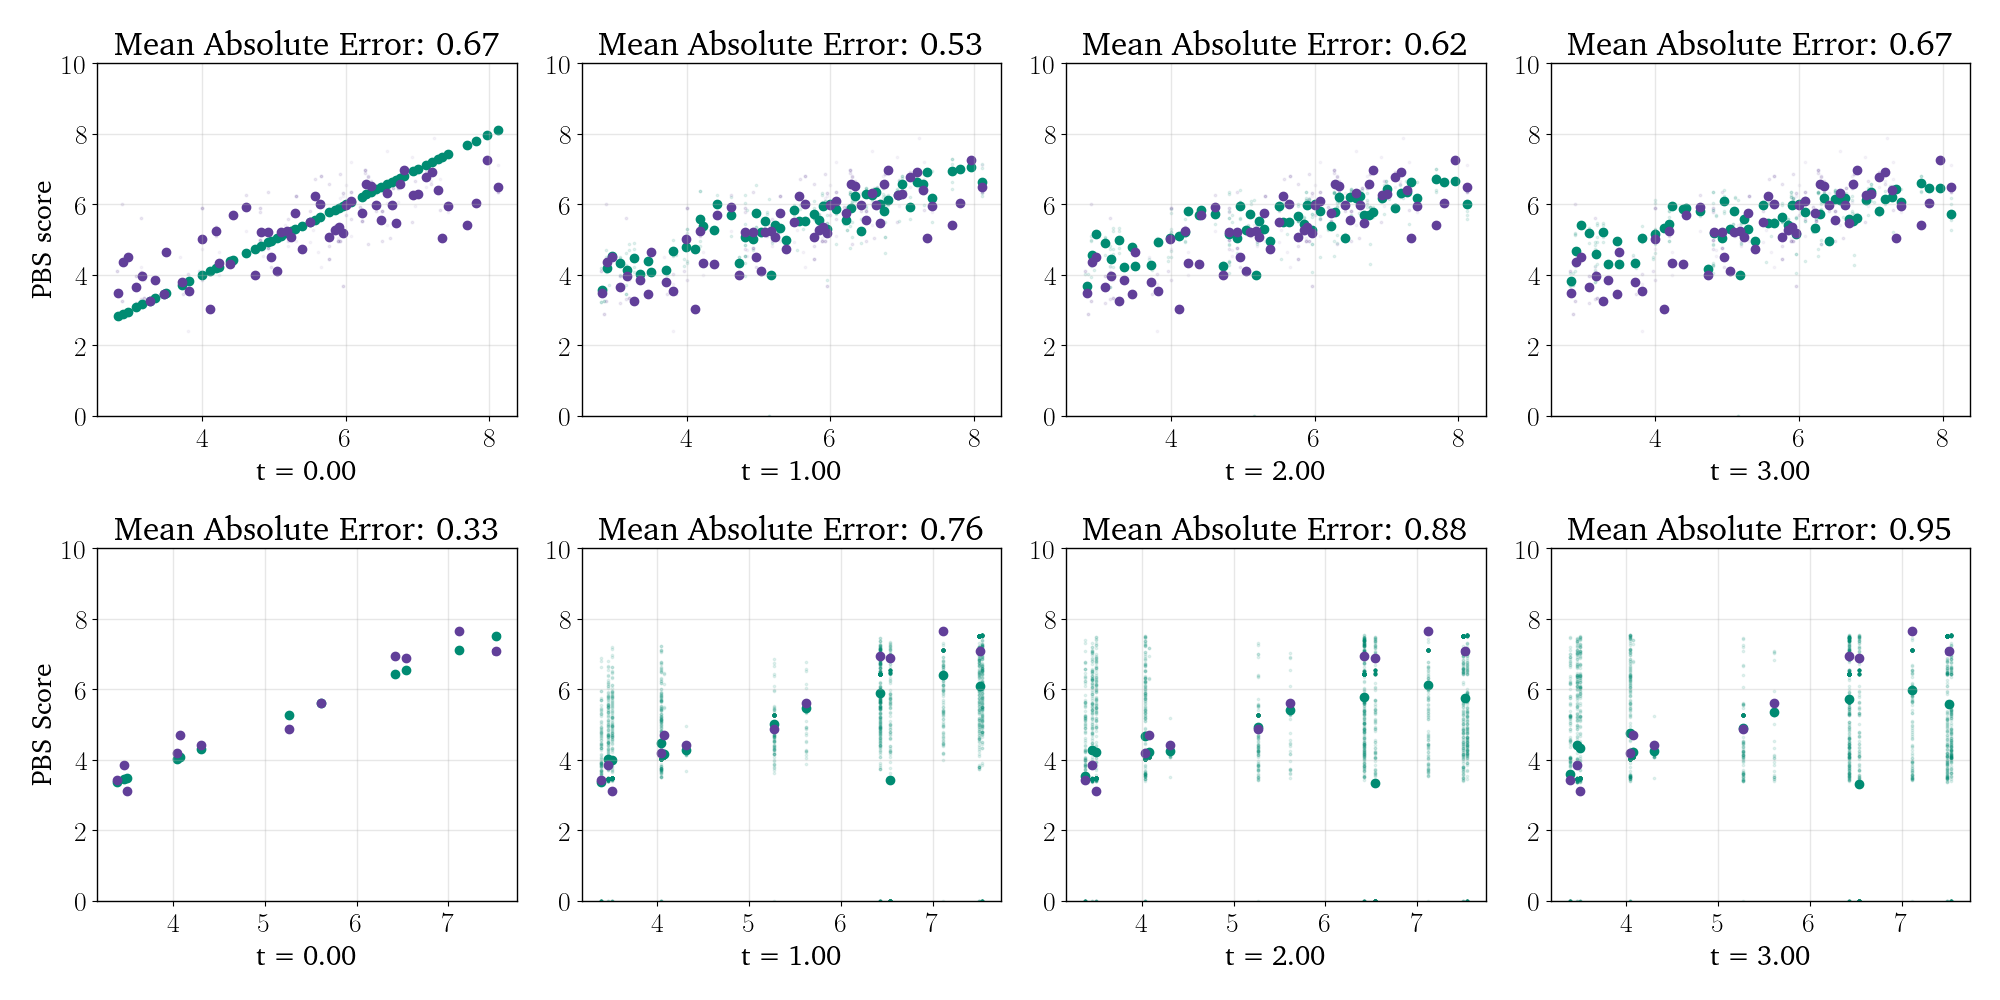
\includegraphics[width=0.95\textwidth]{Figures/pbs_scores.png}
	\end{center}
	\caption{PBS scores, purple indicating the PBS score after deliberation in the original data, green indicates the results of the simulation in that time step.}\label{fig:pbs}
\end{figure}

\Cref{fig:delta_pbs} shows the change in PBS scores for the deliberation group,
the original data shows that most change happens on people with high PBS
scores, become less extreme. The model seems to get this wrong, in showing the
most change for people with low initial PBS scores. This might be because there
is a correlation between PBS score and knowledge (RUN THE STATS), as shown by
\citet{fishkinCanDeliberationHave2024}, most extreme voters, in terms of PBS,
seemed to also be the most knowledgeable, if this was skewed towards voters
with high PBS, then these voters would have more effect on people's opinions in
this model. Looking at the binned errors in \Cref{fig:binned_errors}, we see
that the model performs better when we do not include knowledge, further
indicating that knowledge is a poor predictor of trust, or persuasiveness. Of
course this claim might be weakened by noting that knowledge in this case
relates strictly to institutional knowledge, such as know which party currently
has a majority in the senate. Thus, this specific knowledge might be
insufficient to predict someone's persuasiveness on the topic of immigration for
example.

We note that this slight positive results are only the case when group the
voters by their original positions, thereby giving the model reasonable
predictive power over a population of voters. \Cref{fig:binned_errors} shows
the progression of errors over time when the error is calculated on a
per-individual basis, and we find the model consistently does worse simply predicting someone to not change the opinion at all.

\begin{figure}
	\begin{center}
		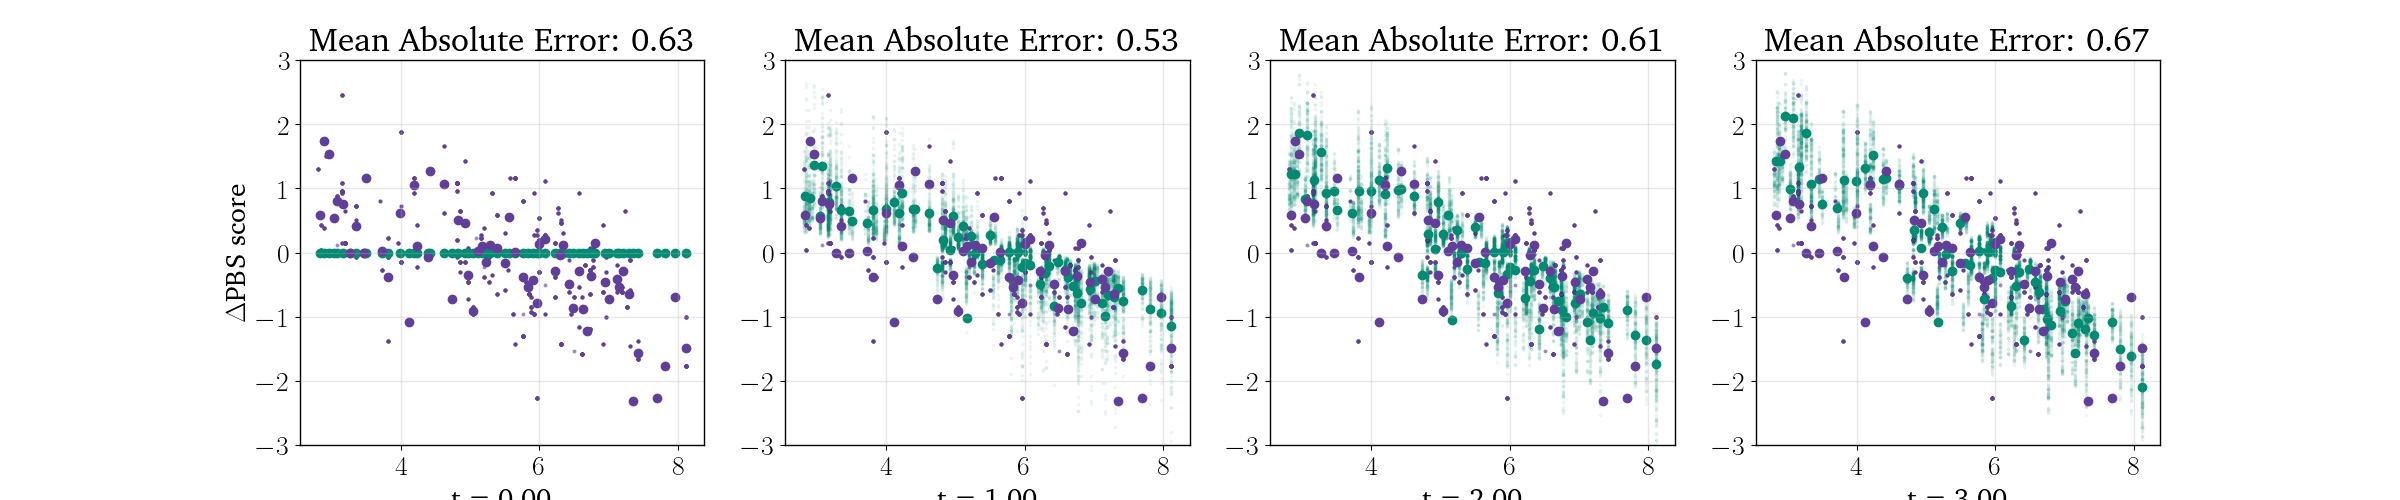
\includegraphics[width=\textwidth]{Figures/change_pbs_scores.png}
	\end{center}
	\caption{Change in PBS score, relative to the original, pre deliberation, measurement. The control is  omitted as there was no significant change.}\label{fig:delta_pbs}
\end{figure}

\Cref{fig:bias_over_time} shows the relation between the bias factor and the PB
score, showing that the bias does not improve the models predictive power. This
result is slightly surprising as one might expect a bias to ``slow down'' the
model. Given that the model does best in early time steps, this slowing down
effect should make the model more stable.


\begin{figure}
	\begin{center}
		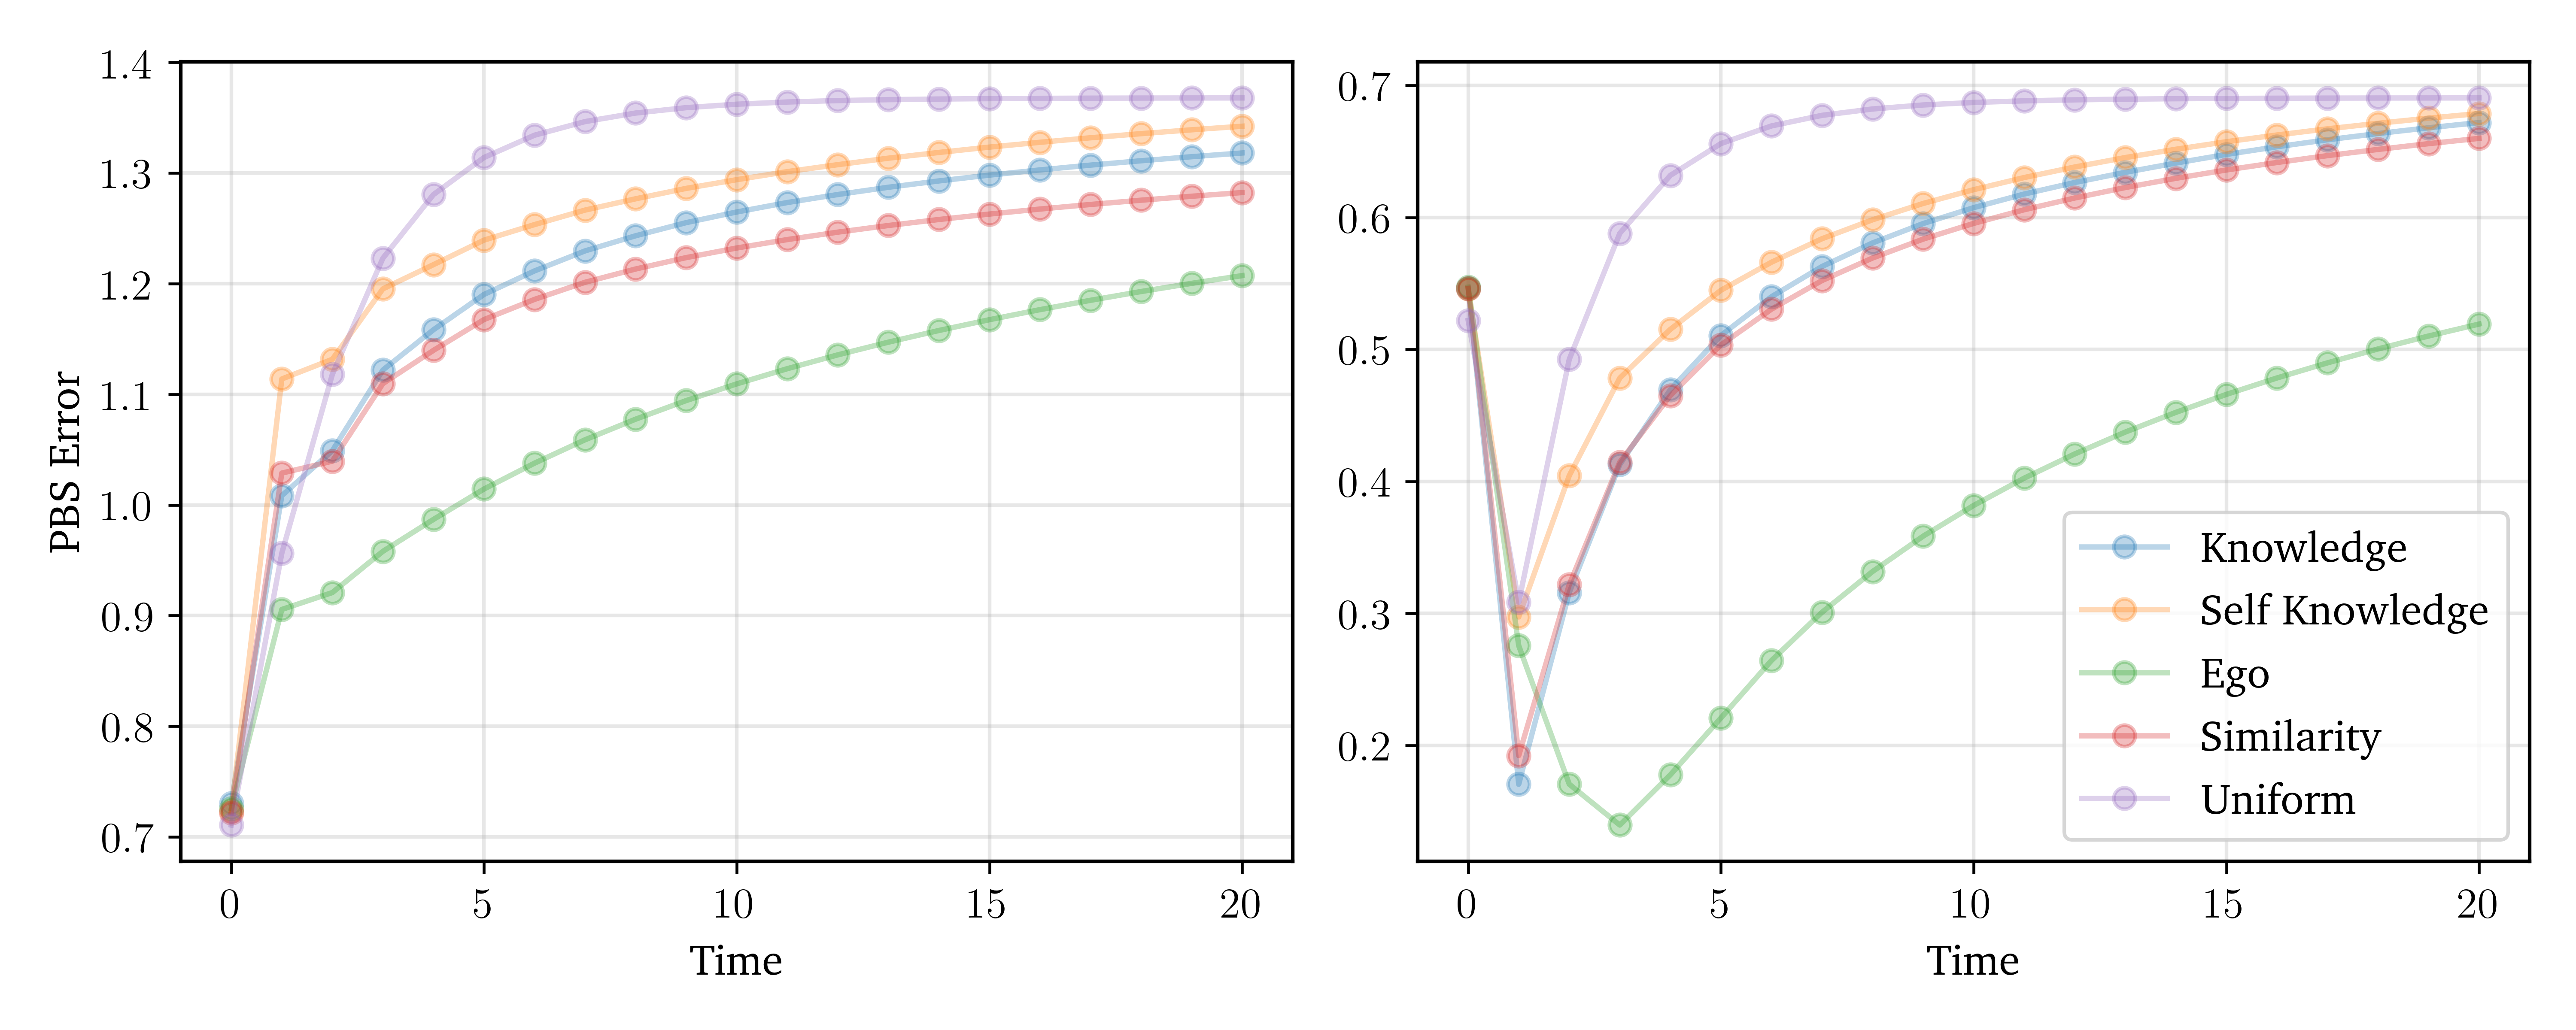
\includegraphics[width=0.95\textwidth]{Figures/errors_binned.png}
	\end{center}
	\caption{Prediction error of the model as a function of time, binned relative to the original PBS scores.}\label{fig:binned_errors}
\end{figure}


\begin{figure}
	\centering

	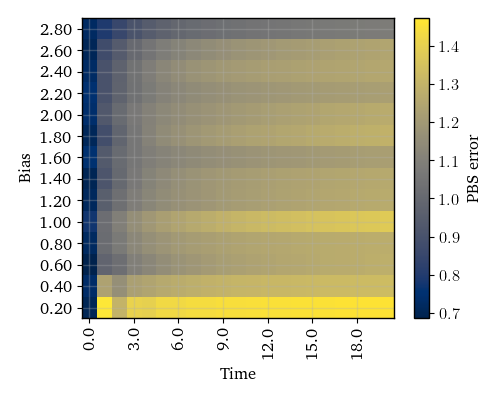
\includegraphics[width=0.6\textwidth]{Figures/bias_time_imshow.png}
	\hspace{1em}
	\caption{PBS Errors as a function of Bias, the horizontal histogram shows the (uniform) distribution of biases, the vertical histogram shows the distribution of MAE of the PBS.}\label{fig:bias_over_time}
\end{figure}


Here it is clear that generally the model performs best when both the number of
candidates and the number of voters are low. We also not that though the error
of the different candidate generators are comparable, they in general the
Sample methods seems to results in larger errors, meaning that the model is
less well able to capture circumstances where the alternative's opinions are
not represented in the deliberating population. Finally, we see that The
distribution of best biases skews to values around 1.3, thus indicating that
even while deliberating, people tend to hold their opinion to be \textit{more}
important than that of all other voters.

We investigate this discrepancy between the two candidates generation methods
now, to this end we look at the difference in error for all tested
configuration.

% Now we T test on everything the Sample and Voter method

\subsection{Convergence}

From \Cref{theory}, we have seen that in the limit some matrices are
convergent, while some are not, in particular if the matrix is aperiodic, this
it is convergent. As we model the deliberation group as having fully connected
matrices, the matrices are aperiodic, and thus convergent. We look at the
distance between the estimated support matrix, and the true support matrix, to
get a sense of the rate of convergence. The distance in the element wise
$\ell_1$ norm.

\begin{figure}
	\begin{center}
		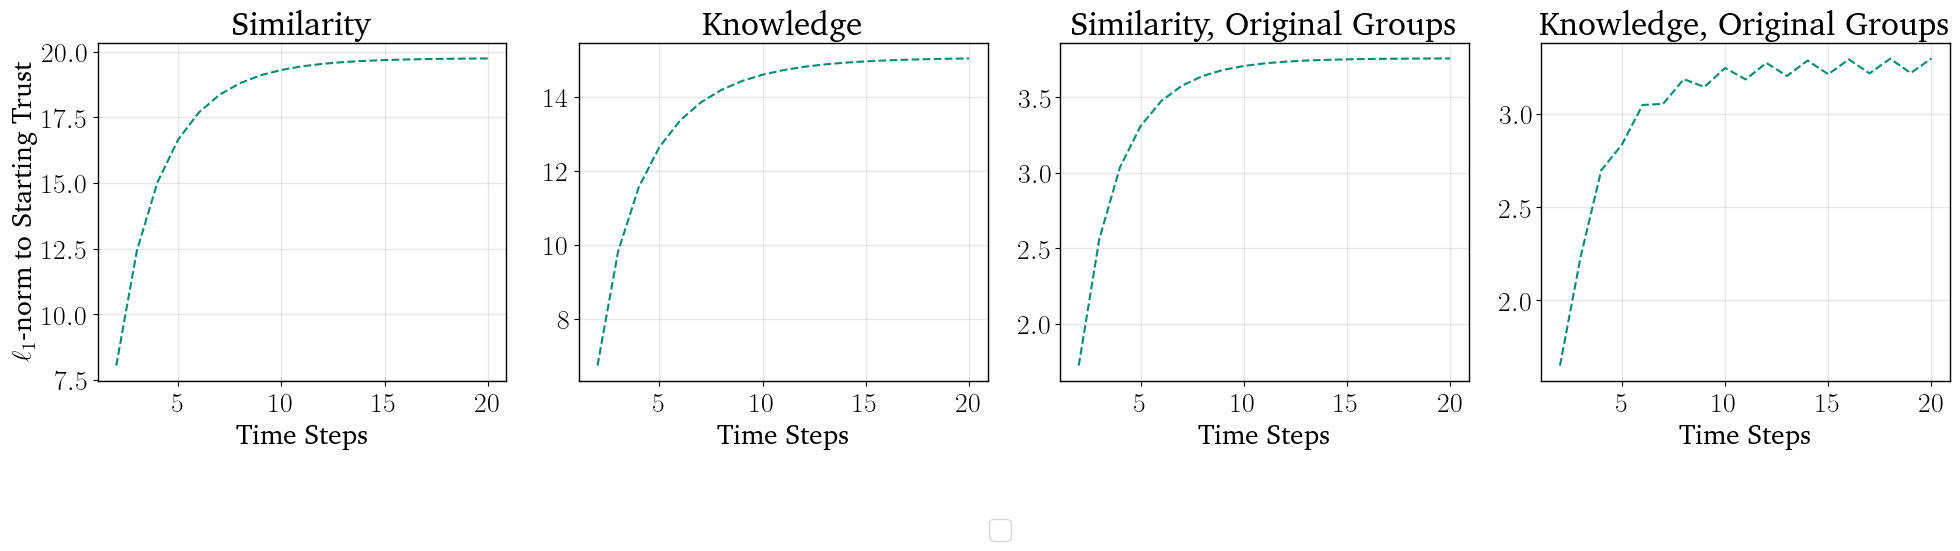
\includegraphics[width=0.95\textwidth]{Figures/convergence_groups.png}
	\end{center}
	\caption{Convergence of different distance metrics as well as the
		$\ell_1$-norm between the trust matrix at the start and time step
		t}\label{fig:convergence_big}
\end{figure}



We now proceed to look at distance to single-peaked profiles, look at both
voter removal and candidate removal. We show that for optimal bias, as
deliberation progresses we see an increase in the proximity to single
peakedness.


\begin{figure}[htbp]
	\centering
	\begin{minipage}{0.45\textwidth}
		\centering
		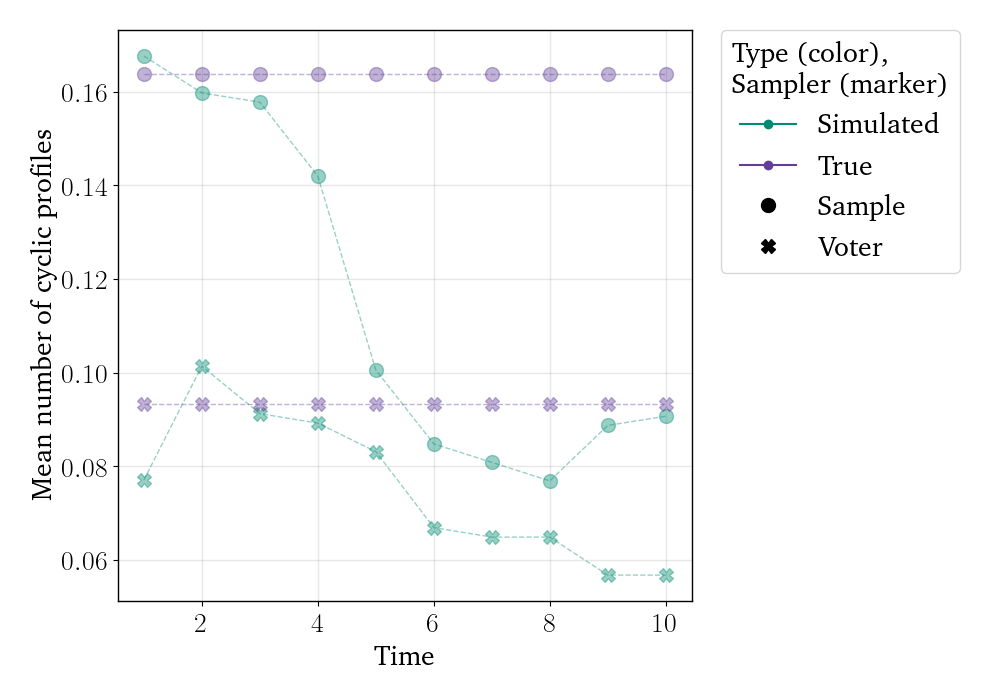
\includegraphics[width=\textwidth]{Figures/delib_Mean Number of Cyclic Profiles.png}
		\caption{The proportion of cyclic profiles remaining, 0 indicating that no cyclic profiles were present after deliberation.}
		\label{fig:degroot_cyclic}
	\end{minipage}\hfill
	\begin{minipage}{0.45\textwidth}
		\centering
		\vspace{-9pt}
		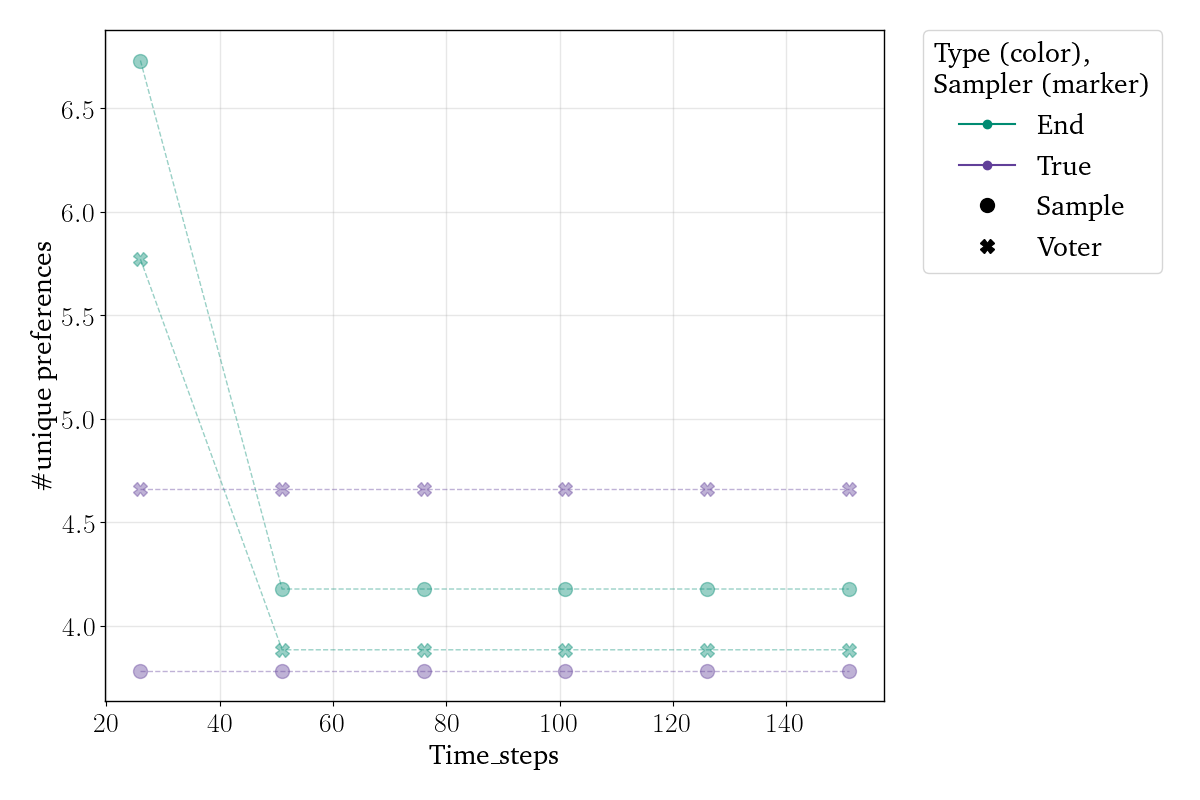
\includegraphics[width=\textwidth]{Figures/delib_number_Unique Preferences.png}
		\caption{Number of unique preferences at the final step of deliberation.}
		\label{fig:degroot_count}
	\end{minipage}

	\vspace{1em}

	\begin{minipage}{0.45\textwidth}
		\centering
		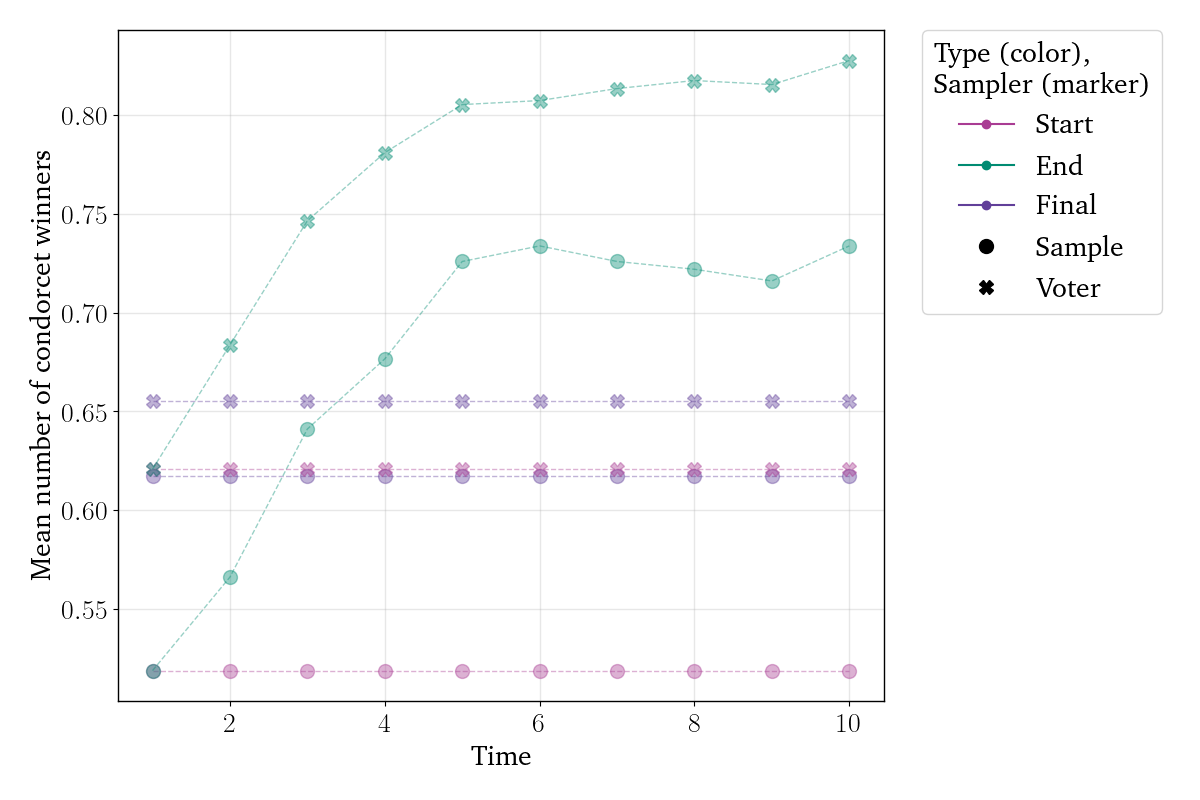
\includegraphics[width=\textwidth]{Figures/delib_Mean number of Condorcet winners.png}
		\caption{The proportion of Condorcet winners left after deliberation, value above one indicate Condorcet winners emerging during deliberation}
		\label{fig:degroot_condorcet}
	\end{minipage}\hfill
	\begin{minipage}{0.45\textwidth}
		\centering
		\vspace{-9pt}
		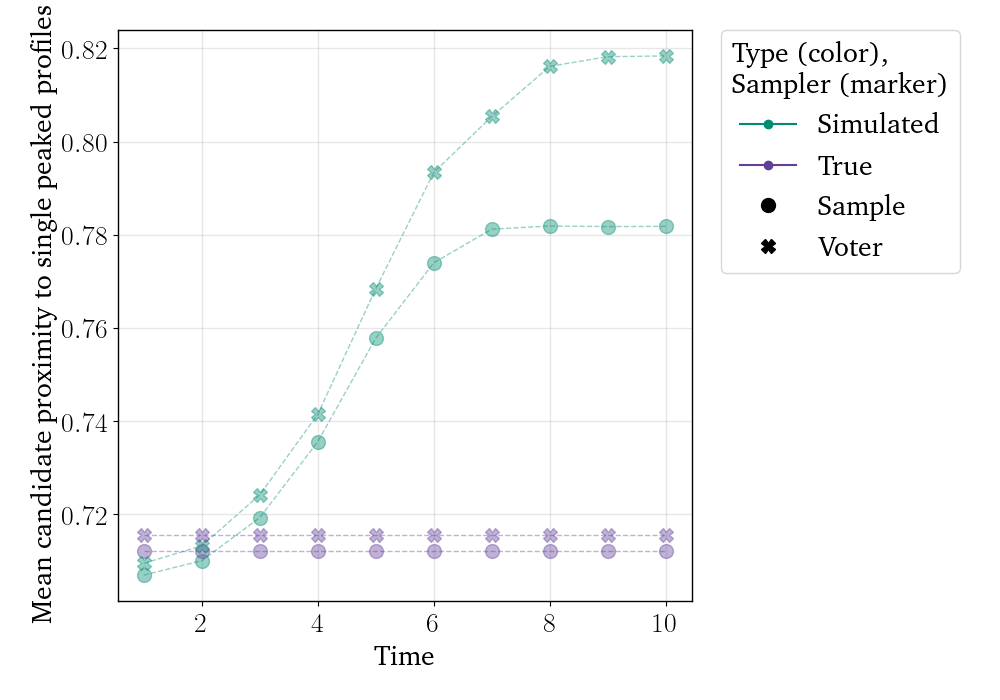
\includegraphics[width=\textwidth]{Figures/delib_Mean candidate proximity to single peaked Profiles.png}
		\caption{Proximity to single-peakedness after deliberation. Proximity to single-peakedness as defined in \Cref{section:related_work}.}
		\label{fig:degroot_single_peaked}
	\end{minipage}
\end{figure}

Between the deliberation group and the control group, if we look at the final
time step, we find that both perform best if the bias is set to be around 1,
though this differs based on the other parameters. This seems to indicate that
for both smaller and larger groups, a voter's opinion is in some sense equally
important as the of  \textit{all} other voters she comes in contact with. In
other words, it does not seem to matter how many people disagree with a voter,
her own opinion holds a constant relative importance.
